% Copyright (c) 2026, Riot Authors. All rights reserved.
%
% Standalone version of the block-AMR mesh illustration from the
% programmer's guide (sections/programmer_guide.tex).
%
% Compile to PDF:  pdflatex amr_mesh_standalone.tex
% Convert to PNG:  pdftoppr / magick / pdftocairo (see accompanying commands)
\documentclass[tikz,border=6pt]{standalone}

\usepackage{tikz}
\usetikzlibrary{calc,decorations.pathreplacing}

% Colors from riot_manual.tex
\definecolor{riotblue}{RGB}{20,70,130}
\definecolor{riotdark}{RGB}{10,15,25}
\definecolor{riotgray}{RGB}{90,90,90}

\begin{document}
  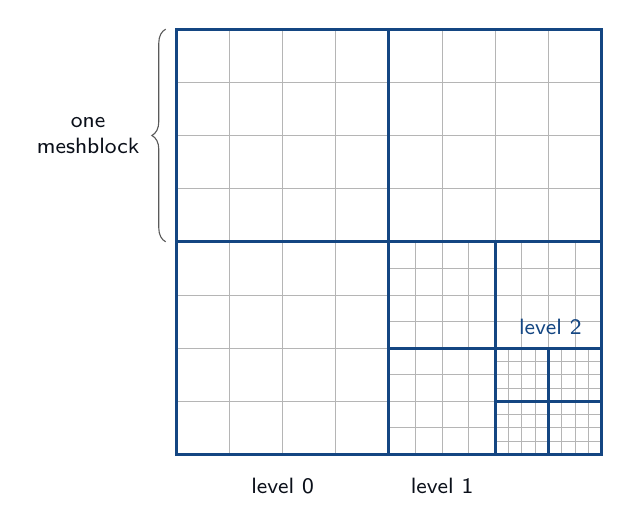
\begin{tikzpicture}[scale=0.9]
    % Style definitions
    \tikzset{
      block/.style={draw=riotblue, line width=1.1pt},
      cell/.style={draw=riotgray!45, line width=0.3pt},
      lbl/.style={font=\footnotesize\sffamily, text=riotdark},
    }
    % ------------------------------------------------------------------
    % Helper macro: draw one meshblock as an nxn grid of cells at
    % (#1,#2) with side length #3, subdivided into #4 cells per side.
    % ------------------------------------------------------------------
    \newcommand{\meshblock}[4]{%
      \begin{scope}[shift={(#1,#2)}]
        \pgfmathsetmacro{\step}{#3/#4}%
        \foreach \i in {1,...,\numexpr#4-1\relax}{%
          \draw[cell] (\i*\step,0) -- (\i*\step,#3);
          \draw[cell] (0,\i*\step) -- (#3,\i*\step);
        }
        \draw[block] (0,0) rectangle (#3,#3);
      \end{scope}%
    }

    % Level 0: three root meshblocks (each 4x4 cells, side 3)
    \meshblock{0}{0}{3}{4}
    \meshblock{0}{3}{3}{4}
    \meshblock{3}{3}{3}{4}

    % Level 1: bottom-right root block refined into 2x2 children
    % (each side 1.5, still 4x4 cells), covering the (3,0)-(6,3) area
    \meshblock{3}{0}{1.5}{4}
    \meshblock{4.5}{0}{1.5}{4}
    \meshblock{3}{1.5}{1.5}{4}
    \meshblock{4.5}{1.5}{1.5}{4}

    % Level 2: the bottom-right level-1 child refined again into 2x2
    % (each side 0.75, 4x4 cells), covering (4.5,0)-(6,1.5)
    \meshblock{4.5}{0}{0.75}{4}
    \meshblock{5.25}{0}{0.75}{4}
    \meshblock{4.5}{0.75}{0.75}{4}
    \meshblock{5.25}{0.75}{0.75}{4}

    % Level annotations
    \node[lbl] at (1.5,-0.45) {level 0};
    \node[lbl] at (3.75,-0.45) {level 1};
    \node[lbl, text=riotblue] at (5.25,1.5+0.30) {\,level 2};

    % Bracket callout for a single meshblock (top-left root block)
    \draw[decorate, decoration={brace, amplitude=5pt}, riotgray]
      (-0.15,3) -- (-0.15,6) node[midway, left=6pt, lbl, align=center]
      {one\\meshblock};
  \end{tikzpicture}
\end{document}
